\documentclass[tikz,border=10pt]{standalone}
\usepackage{amsmath,amssymb}
\usepackage{tikz}
\usepackage{pgfplots}
\pgfplotsset{compat=1.18}
\usetikzlibrary{arrows.meta,calc,patterns,positioning,shapes,decorations.markings,backgrounds,fit,intersections}

% Atlas colors
\definecolor{AtlasTeal}{HTML}{5BA4A4}
\definecolor{AtlasTealDark}{HTML}{4A8F8F}
\definecolor{AtlasTealLight}{HTML}{E8F4F4}
\definecolor{AtlasDeep}{HTML}{2C5F5F}
\definecolor{AtlasSage}{HTML}{7BAE7F}
\definecolor{AtlasSageLight}{HTML}{EDF5EE}
\definecolor{AtlasWarm}{HTML}{D4A853}
\definecolor{AtlasWarmLight}{HTML}{FDF6E8}

\begin{document}
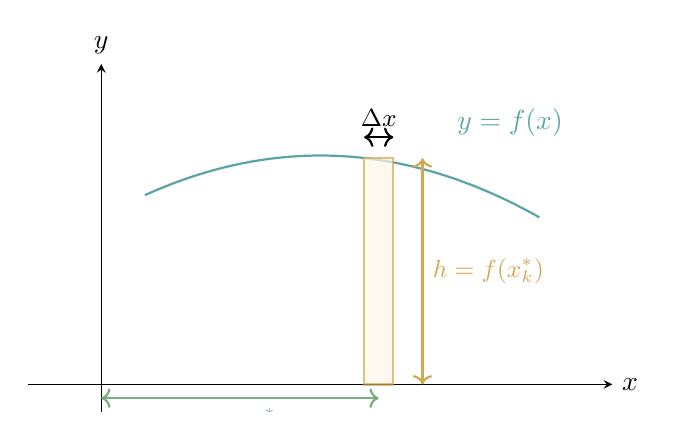
\begin{tikzpicture}
  \begin{axis}[
    width=9cm, height=6cm,
    axis lines=middle,
    xlabel={$x$}, ylabel={$y$},
    xtick=\empty, ytick=\empty,
    xmin=-0.5, xmax=3.5, ymin=-0.3, ymax=3.5,
    every axis x label/.style={at={(ticklabel* cs:1)}, anchor=west},
    every axis y label/.style={at={(ticklabel* cs:1)}, anchor=south},
  ]
    % Curve
    \addplot[AtlasTeal, thick, samples=100, domain=0.3:3] 
      {2.5 - 0.3*(x-1.5)^2};
    
    % A single shell (thin rectangle representing the shell)
    \draw[AtlasWarm, thick, fill=AtlasWarmLight, opacity=0.7] 
      (axis cs:1.8,0) rectangle (axis cs:2.0,2.47);
    
    % Radius annotation
    \draw[<->, thick, AtlasSage] (axis cs:0,-0.15) -- 
      node[below, font=\small] {$r = x_k^*$} (axis cs:1.9,-0.15);
    
    % Height annotation
    \draw[<->, thick, AtlasWarm] (axis cs:2.2,0) -- 
      node[right, font=\small] {$h = f(x_k^*)$} (axis cs:2.2,2.47);
    
    % Thickness
    \draw[<->, thick] (axis cs:1.8,2.7) -- 
      node[above, font=\small] {$\Delta x$} (axis cs:2.0,2.7);
    
    \node[above, AtlasTeal] at (axis cs:2.8,2.6) {$y = f(x)$};
  \end{axis}
\end{tikzpicture}
\end{document}
